\documentclass{beamer}
\usepackage[english]{babel}
\usepackage[utf8]{inputenc}

\usepackage{color}
\usepackage{graphicx}
\usepackage{fancybox}


% for tick marks
%\usepackage{dingbat}

\usepackage{beamerthemesplit}
\usetheme[compress]{MPIjast}


\title[title in footline]{Toponym Resolution and Adaptive Context Features}
\subtitle{}
\author[name in footline]{Faraz Ahmad}
\date{\today}
\institute[MPI-Inf]{
Max Planck Institute for Informatics\\
Saarland Informatics Campus\\
\color{MPIIblue}{s8faahma@stud.uni-saarland.de}}

%---------------------------------------%
%---------- RECURRING OUTLINE ----------%
% have this if you'd like a recurring outline
\AtBeginSection[]  % "Beamer, do the following at the start of every section"
{
\begin{frame}<beamer> 
\frametitle{Outline} % make a frame titled "Outline"
\tableofcontents[currentsection,hideallsubsections]  % show TOC and highlight current section
\end{frame}
}
%----------------------------------------


\begin{document}
\frame[plain]{\titlepage}
\frame{\frametitle{Outline}\tableofcontents[hideallsubsections]}

%========================================
%========================================

\section[Introduction]{Introduction}

%###############################################
\subsection{Important things to understand}

\frame{
	\frametitle{Important things to understand}
	
	\begin{itemize}
		\item Toponyms
		\item Geotagging
		\begin{itemize}
			\item Toponym recognition
			\item Toponym disambiguation
		\end{itemize}
		\item Context Free and Adaptive Context features 
		\item Adaptive features - and their computation
		\item Applications of Geotagging
	\end{itemize}
} % END OF FRAME
%###############################################

%----------------------------------------


\subsection{Terminology}

\frame{
\frametitle{Terminology}

\begin{itemize}
\item Toponyms
\item Geotagging
\begin{itemize}
	\item Toponym recognition
	\item Toponym disambiguation
\end{itemize}
\item Difficulty in Geotagging
\item Gazeteers
\end{itemize}
} % END OF FRAME

%----------------------------------------

\subsection{Toponyms}
\frame{
\frametitle{Toponyms}
\begin{block}{Toponyms}
	Words in a document text/sentence that correspond to a location name are called toponyms.
\end{block}

\begin{block}{refer to a populated place, such as: }
	\begin{itemize}
		\item[(1)] Cities/Towns
		\item[(2)] States/Provinces
		\item[(3)] Countries
	\end{itemize}
\end{block}
} % END OF FRAME

%----------------------------------------

\frame[t]{
\frametitle{Toponyms - examples}

\begin{block}{Toponyms examples: }
	\begin{itemize}
		\item[(1)]  ``\underline{France} won the world cup in 1998."
		\item[(2)] ``\underline{Birmingham}, a major city of \underline{West Midlands} is the second most populous city of \underline{England}, third most populous is \underline{Leeds}."
	\end{itemize}
\end{block}

\begin{columns}
	\begin{column}{.5\textwidth}
		\begin{figure}
			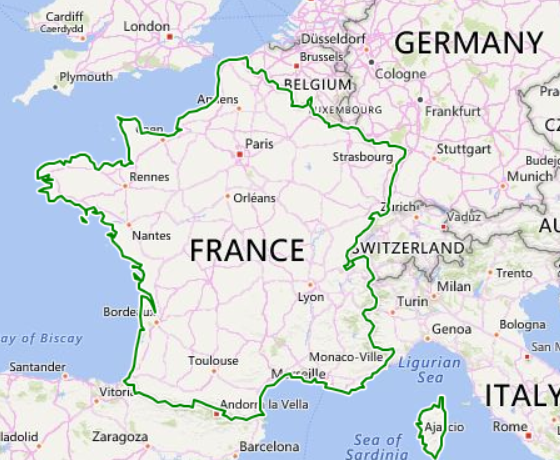
\includegraphics[width=\textwidth]{france.png} 
			%\caption{AvH in Wikipedia, \textit{Source: URL}}
		\end{figure}
	\end{column}
	\begin{column}{.5\textwidth}
		\begin{figure}
			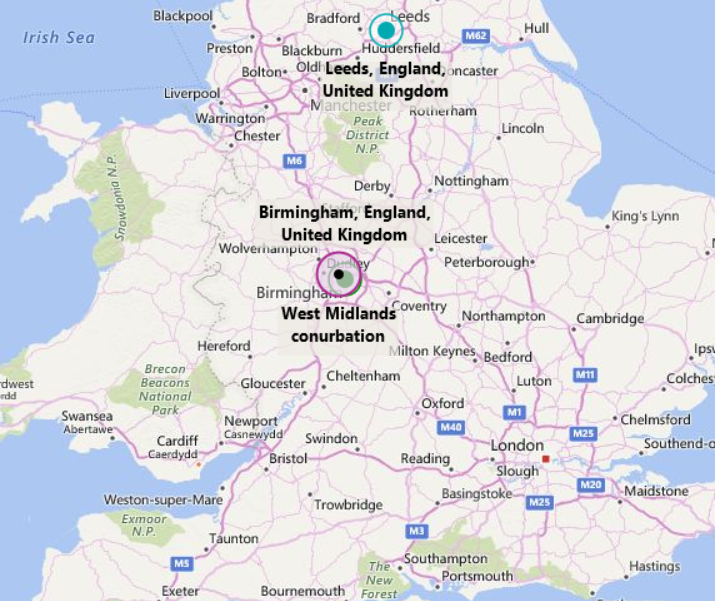
\includegraphics[width=\textwidth]{uk.png} 
			%\caption{AvH in Wikipedia, \textit{Source: URL}}
		\end{figure}
	\end{column}
	
\end{columns}

\vfill
} % END OF FRAME

%========================================

\subsection{Geotagging}


\frame{
\frametitle{Geotagging}

\begin{block}{Geotagging}
	Geotagging means understanding the geographic content of a text document.
\end{block}

\begin{block}{is a two step process: }
	\begin{itemize}
		\item[(1)] detecting the toponyms
		\item[(2)] grounding the detected toponyms
	\end{itemize}
\end{block}

\vfill
} % END OF FRAME

%----------------------------------------

\frame{
\frametitle{Geotagging - example}
\begin{block}{sentence }
	``France won the world cup in 1998."
\end{block}
\begin{block}{step 1: detecting the toponyms}
	``\underline{France} won the world cup in 1998."
\end{block}
\begin{block}{step 2: grounding the detected toponyms}
``\underline{France}(lat 46, long 2) won the world cup in 1998."
\end{block}

\vfill
} % END OF FRAME

%----------------------------------------

\frame{
	\frametitle{Geotagging - the two steps defined}
	
	\begin{itemize}
		\item Toponym recognition (Geoparsing)
		\item Toponym resolution (Geocoding)
	\end{itemize}
	 
	 
	\begin{block}{Toponym recognition}
		aims to find all the toponyms(location
		names) in text.
	\end{block}
	\begin{block}{Toponym resolution}
		aims to resolve the ambiguity in toponyms as one location name can refer to multiple location names
		in the world, so the aim of toponym resolution is to assign the correct lat/long value to a toponym.
	\end{block}
	
	\vfill
} % END OF FRAME

%----------------------------------------

\frame{
	\frametitle{Geotagging - example}
	\begin{block}{sentence }
		``France won the world cup in 1998."
	\end{block}
	\begin{block}{step 1: detecting the toponyms = Toponym recognition}
		``\underline{France} won the world cup in 1998."
	\end{block}
	\begin{block}{step 2: grounding the detected toponyms = Toponym resolution}
		``\underline{France}(lat 46, long 2) won the world cup in 1998."
	\end{block}
	
	\vfill
} % END OF FRAME

%========================================

\subsection{Difficulty in Geotagging}


\frame{
\frametitle{Difficulty in Geotagging}

\begin{block}{in toponym recognition}
	need to understand natural language in order to detect toponyms accurately.
\end{block}

\begin{block}{in toponym resolution}
	need to understand document's content to ground a toponym to its correct lat/long value\textbf{(correct interpretation)}.
\end{block}


} % END OF FRAME

\subsection{Difficulty in Geotagging - example}


\frame{
	\frametitle{Difficulty in Geotagging - ambiguity}
	
	\begin{block}{geo/geo ambiguity}
		An example for ambiguous geographic term can be \textbf{"Hyderabad"}, it is a city in Pakistan and India.
	\end{block}
	
	\pause
	
	\begin{block}{geo/non-geo ambiguity}
		Another example for ambiguous geographic term can be \textbf{"Jordan"}, it is a name of a country and a person
	\end{block}
	
	
} % END OF FRAME
%========================================

\subsection{Gazeteers}


\frame{
	\frametitle{Gazeteers}
	
	\begin{block}{Gazeteers}
		Gazeteers are long lists of geographic locations with respective features such as lat/long values and usually type of location(city, state, country etc).
	\end{block}

	\begin{block}{some examples of online available gazeteers}
		\begin{itemize}
			\item GeoNames
			\item World Factbook by CIA
			\item Getty Thesaurus of Geographic Names
		\end{itemize}	
	\end{block}
	
} % END OF FRAME

%----------------------------------------

\frame{
	\frametitle{Gazeteers}
	
	\begin{block}{useful for}
		\begin{itemize}
			\item Toponym recognition (looking up)
			\item getting features* of toponyms 
			\item lat/long value of the toponym
		\end{itemize}
	\end{block}
	
	$\ast$ population, no. of interpretations, alternative names, location type
	
	\begin{figure}
		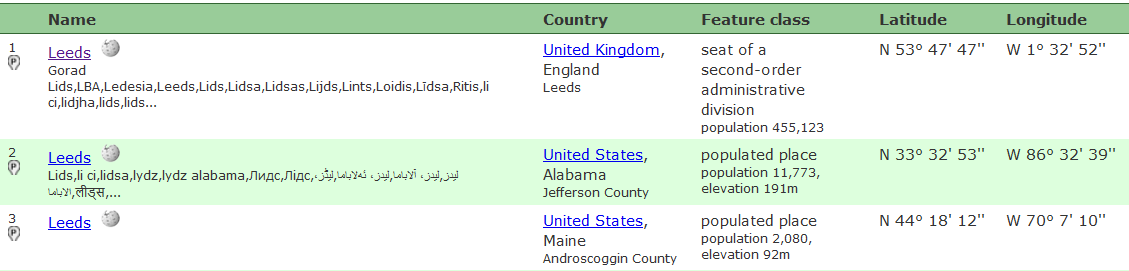
\includegraphics[width=\textwidth]{geonames.png} 
		\caption{GeoNames gazeteer}
	\end{figure}
		
} % END OF FRAME

%========================================
%========================================

\section[Motivation]{Motivation}


\subsection{Geographic content in queries}

\frame{
	\frametitle{Geographic content in queries}
	
	\begin{itemize}
		\item 14.8\% geographic queries in 2001 Excite search engine log
		\item 13\% geographic queries(related to USA) in 3 months data of AOL search engine in 2006 
	\end{itemize}
	
	
} % END OF FRAME

%----------------------------------------


%========================================
%========================================



\subsection{NERD vs Geotagging}


\frame{
\frametitle{NERD vs Geotagging}

\begin{columns}
	\begin{column}{.5\textwidth}
			\alert{NERD}
			\begin{itemize}
				\item disambiguate all entities
				\item uses knowledgebases to ground entities
				\item ground = link to the correct knowledgebase entry about entity
			\end{itemize}
	\end{column}
	\begin{column}{.5\textwidth}
			\alert{Geotagging}
			\begin{itemize}
				\item disambiguate only toponyms
				\item uses various features to ground toponyms
				\item ground = assign correct lat/long value to the toponym
			\end{itemize}
	\end{column}
\end{columns}

\pause

\begin{block}{Bottom line}
	Geotagging deserves attention in its own right, and NERD cannot be used for it.
\end{block}

\vfill
} % END OF FRAME

%----------------------------------------
%========================================


\section[Adaptive Context Features]{Adaptive Context Features}

\subsection{Toponym recognition procedure}
\frame{
	\frametitle{Toponym recognition procedure}
	
	\begin{itemize}
		\item tokenization
		\item lookups
		\item statistical NLP tools
		\item POS tagging
	\end{itemize}
} % END OF FRAME
%----------------------------------------

\subsection{Toponym resolution procedure}
\frame{
	\frametitle{Toponym resolution procedure}
	
	\begin{itemize}
		\item cast as classification problem
		\item identify each toponym/interpretation pair as correct or incorrect
		\item used decision trees
		\item can get confidence score for each decision
	\end{itemize}
\vfill
} % END OF FRAME
%----------------------------------------

\subsection{Input features }
\frame{
	\frametitle{Input features for resolution}
	
	\begin{itemize}
		\item Context free features
		\item Adaptive context features
	\end{itemize}

	\pause

	\begin{block}{Context free features}
		 do not depend on the context(window) of the toponym t being resolved; usually available from gazeteers
	\end{block}

	\pause
	
	\begin{block}{Adaptive context features}
		depend on the context(window) around the toponym t being resolved; other toponyms in the window	around toponym t help in resolving it
	\end{block}
\vfill
} % END OF FRAME
%----------------------------------------

\subsection{Context Free Features}
\frame{
	\frametitle{Context Free Features}
	
	\begin{itemize}
		\item Interpretations
		\item Population
		\item Altnames
		\item Dateline
		\item Locallex
	\end{itemize}
} % END OF FRAME
%----------------------------------------

\subsection{Adaptive Context Features}
\frame{
	\frametitle{Adaptive Context Features}
	
	\begin{block}{Context of a toponym t}
	means that other toponyms in the window around toponym t
	\end{block}

	\begin{overprint}
		\onslide<1>
		\begin{figure}
			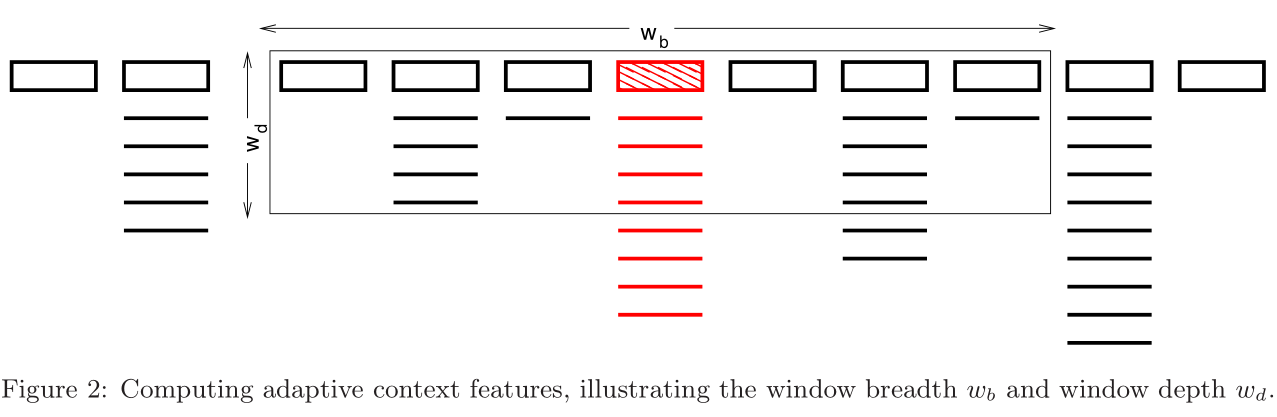
\includegraphics[width=\textwidth]{adaptive.png} 
			\caption{from Lieberman and Samet, \textit{Source: URL}}
		\end{figure}
					
	\end{overprint}

} % END OF FRAME
%----------------------------------------

\frame{
	\frametitle{Adaptive Context Features}
	
	\begin{block}{Adaptive}
		means that the window's breadth $w_b$ and depth $w_d$ can be changed
	\end{block}
	
	%\begin{block}{Depth $w_d$ of window}
	%	the number of interpretations to consider for each toponym in the window
	%\end{block}
	
	\begin{overprint}
		\onslide<1>
		\begin{figure}
			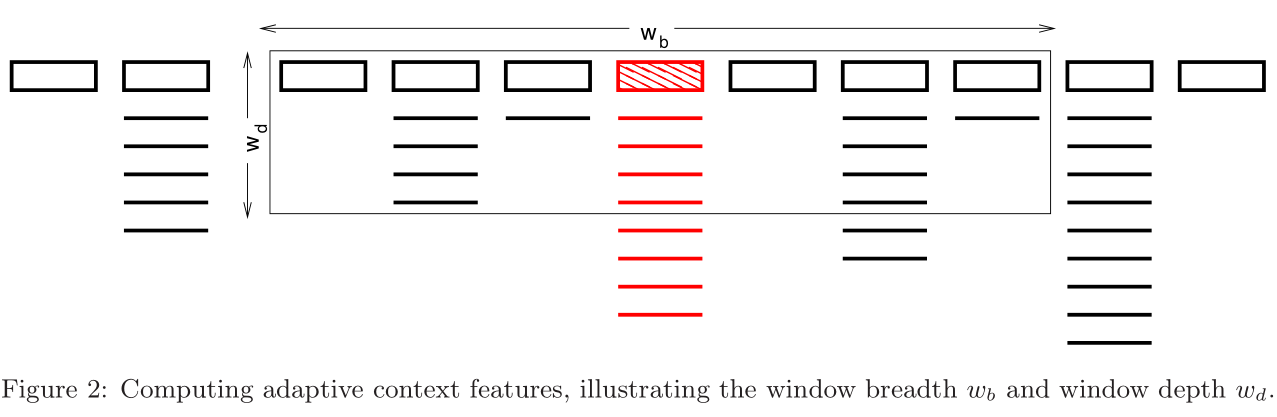
\includegraphics[width=\textwidth]{adaptive.png} 
			\caption{from Lieberman and Samet, \textit{Source: URL}}
		\end{figure}
		
		\onslide<2>
		\begin{figure}
			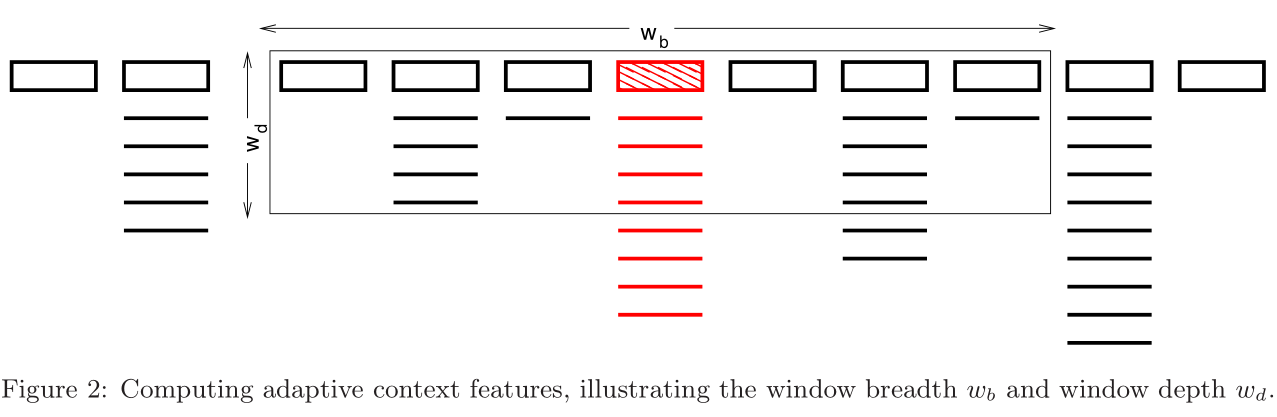
\includegraphics[width=\textwidth]{adaptive.png} 
			\caption{from Lieberman and Samet, \textit{Source: URL}}
		\end{figure}
		
		\vspace*{-5cm}
		\begin{block}{\centering advantage of adaptiveness}
			\centering {$w_b$ and $w_d$ can be changed to make the resolution process faster or more accurate!}
		\end{block}
		
	\end{overprint}
	
} % END OF FRAME
%----------------------------------------

\subsection{1. Proxmity Features}
\frame{
	\frametitle{1. Proximity Features}
	
	\begin{block}{1. Proximity Features}
		represent the average distance of an interpretation $l_t$ of toponym $t$, to the geographically closest interpretations, say $l_o$ of all the other toponyms $o$ in the window.
	\end{block}
		\begin{overprint}
		\onslide<1>
		\begin{figure}
			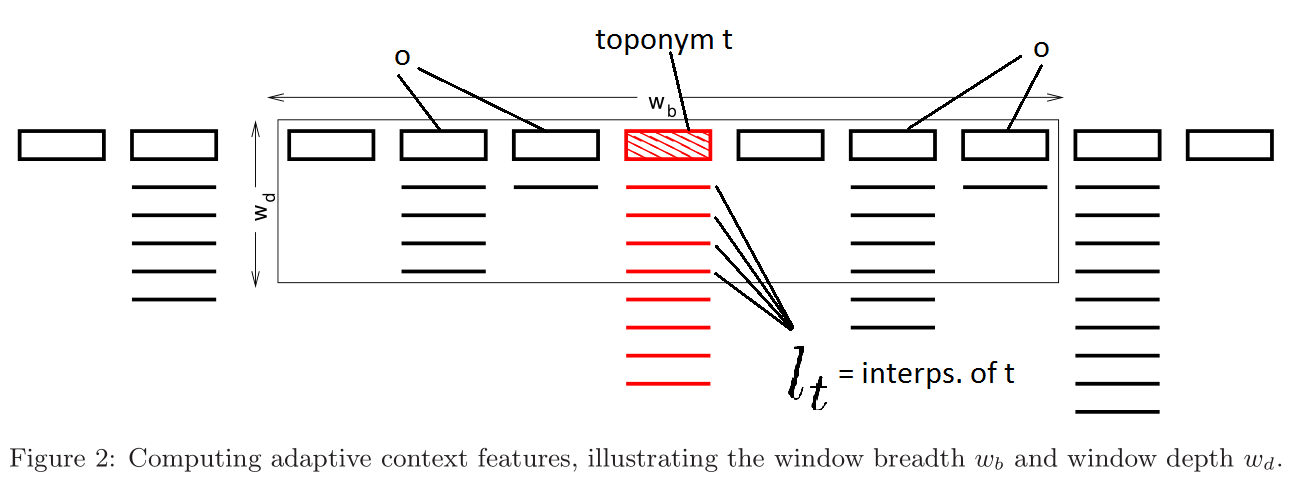
\includegraphics[width=\textwidth]{adaptive-proximity-0.png} 
			\caption{from Lieberman and Samet, \textit{Source: URL}}
		\end{figure}
		
		
	\end{overprint}
} % END OF FRAME
%----------------------------------------

\subsection{Computing Proximity Features}
\frame{
	\frametitle{Computing Proximity Features}
	
	\begin{overprint}
		\onslide<1>
		\begin{figure}
			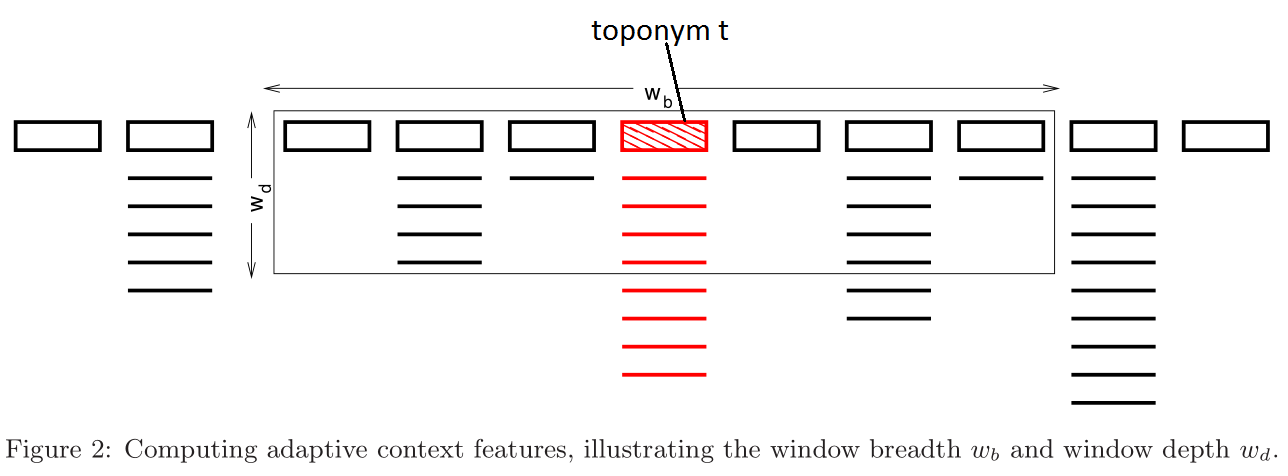
\includegraphics[width=\textwidth]{adaptive-proximity.png} 
			\caption{from Lieberman and Samet, \textit{Source: URL}}
		\end{figure}
		
		\onslide<2>
		\begin{figure}
			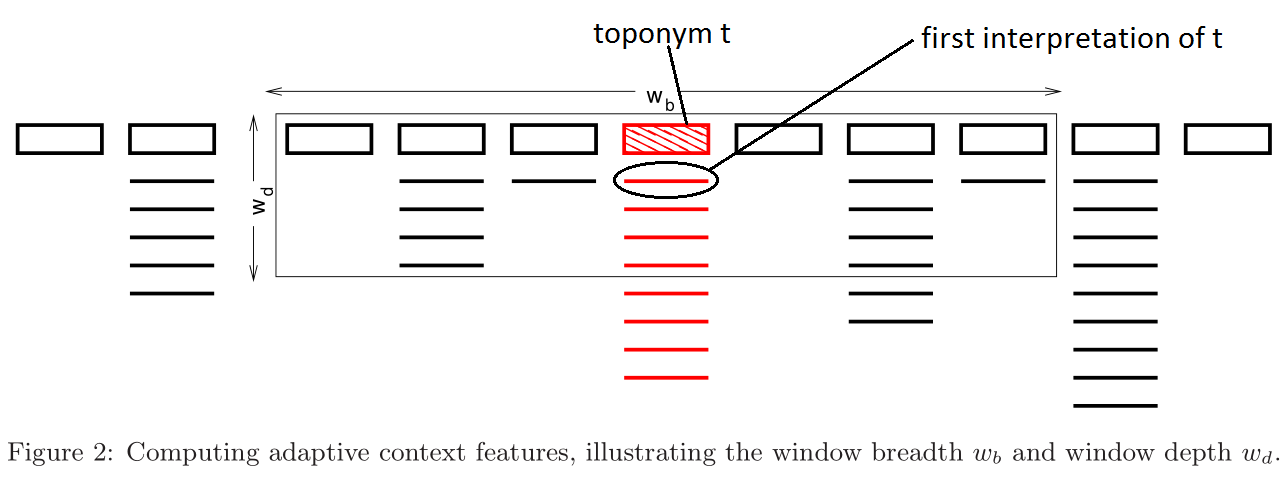
\includegraphics[width=\textwidth]{adaptive-proximity-a.png} 
			\caption{from Lieberman and Samet, \textit{Source: URL}}
		\end{figure}
		
		\onslide<3>
		\begin{figure}
			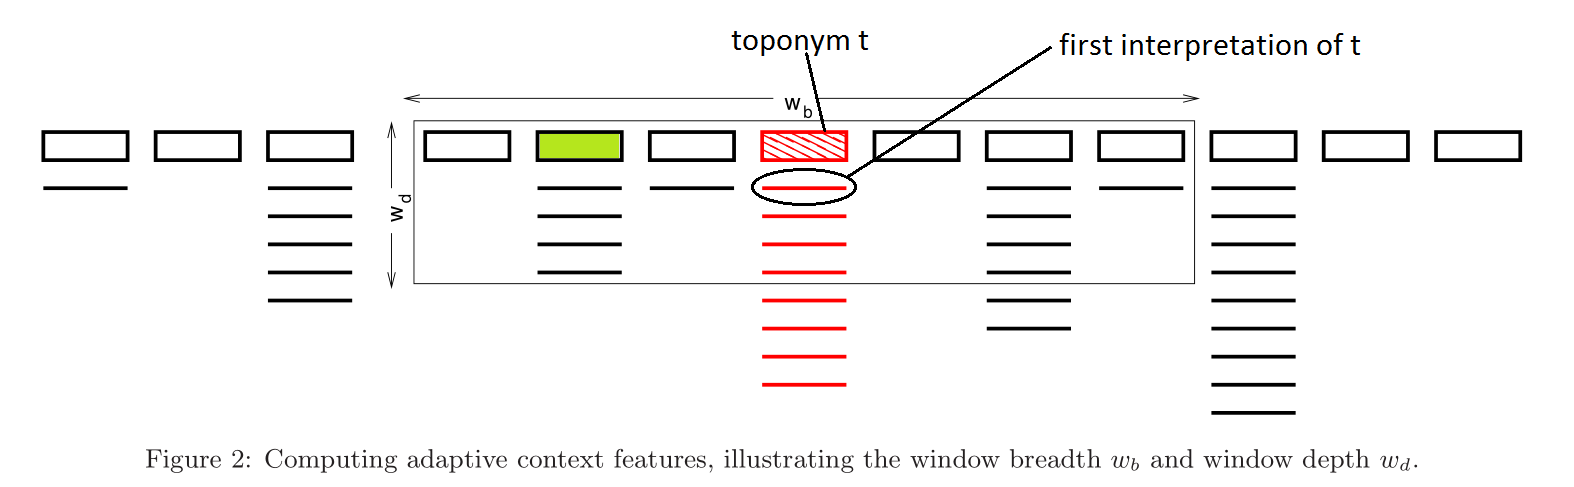
\includegraphics[width=\textwidth]{adaptive-proximity-b.png} 
			\caption{from Lieberman and Samet, \textit{Source: URL}}
		\end{figure}
		
		\onslide<4>
		\begin{figure}
			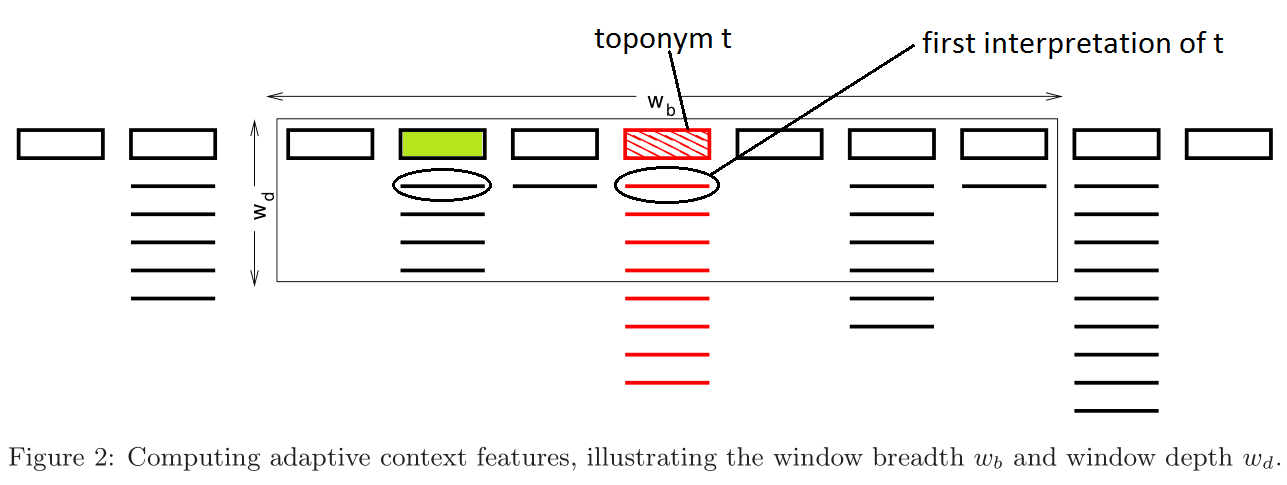
\includegraphics[width=\textwidth]{adaptive-proximity-c.png} 
			\caption{from Lieberman and Samet, \textit{Source: URL}}
		\end{figure}
		
		\onslide<5>
		\begin{figure}
			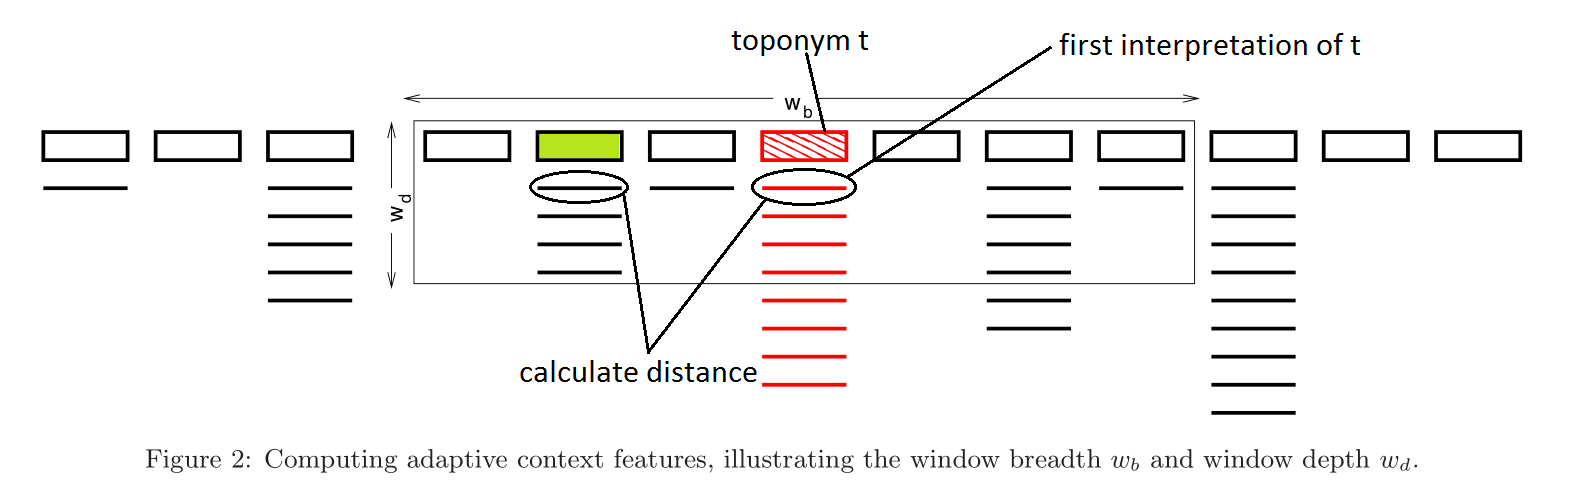
\includegraphics[width=\textwidth]{adaptive-proximity-d.png} 
			\caption{from Lieberman and Samet, \textit{Source: URL}}
		\end{figure}
		
		\onslide<6>		
		\begin{figure}
			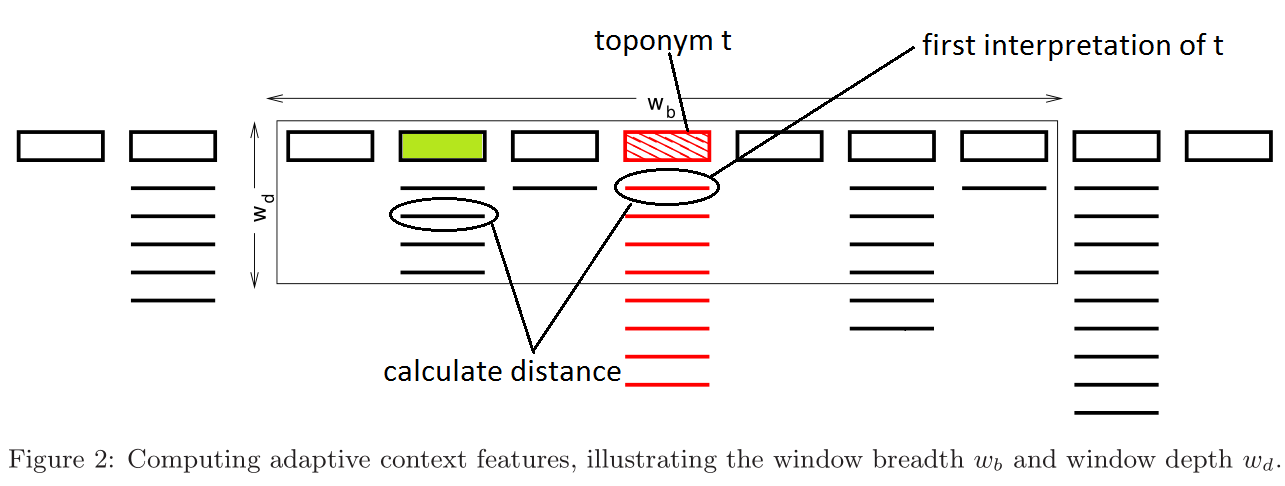
\includegraphics[width=\textwidth]{adaptive-proximity-e.png} 
			\caption{from Lieberman and Samet, \textit{Source: URL}}
		\end{figure}
		
		\onslide<7>
		\begin{figure}
			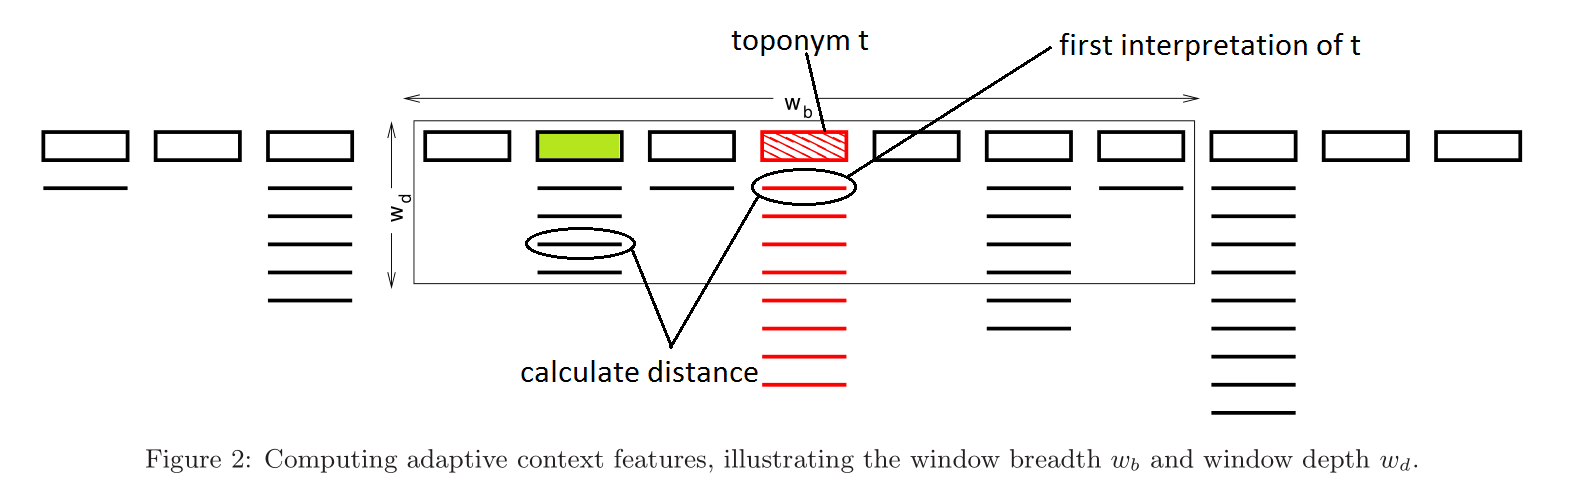
\includegraphics[width=\textwidth]{adaptive-proximity-f.png} 
			\caption{from Lieberman and Samet, \textit{Source: URL}}
		\end{figure}
		
		\onslide<8>
		\begin{figure}
			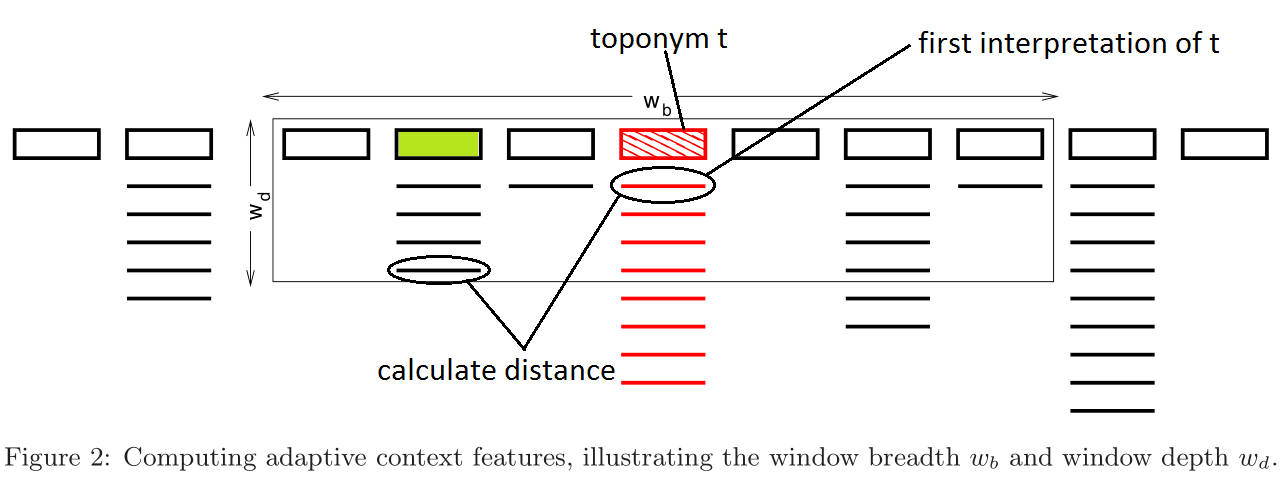
\includegraphics[width=\textwidth]{adaptive-proximity-g.png} 
			\caption{from Lieberman and Samet, \textit{Source: URL}}
		\end{figure}
		
		\onslide<9>
		\begin{figure}
			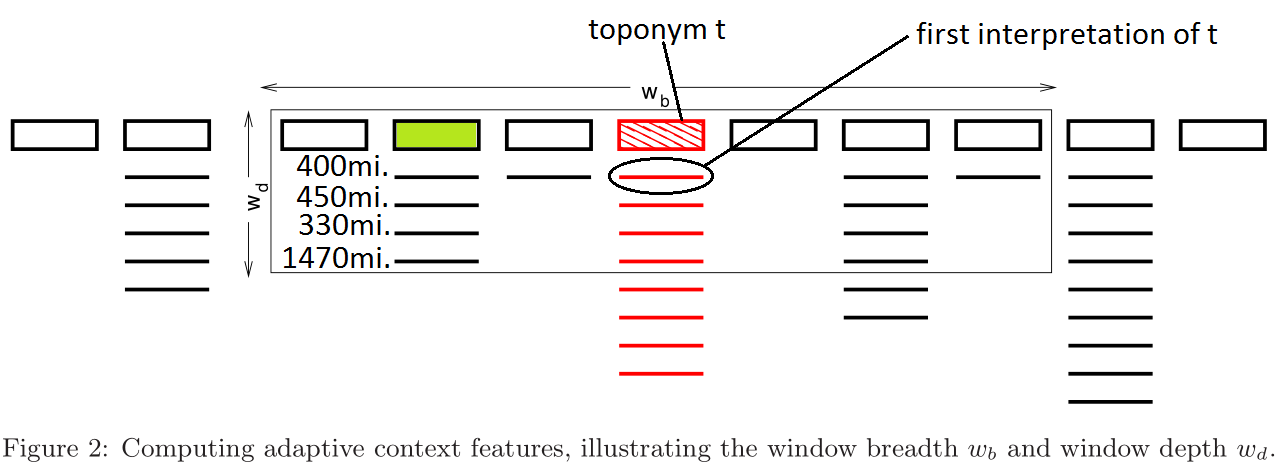
\includegraphics[width=\textwidth]{adaptive-proximity-h.png} 
			\caption{from Lieberman and Samet, \textit{Source: URL}}
		\end{figure}
		
		\onslide<10>
		\begin{figure}
			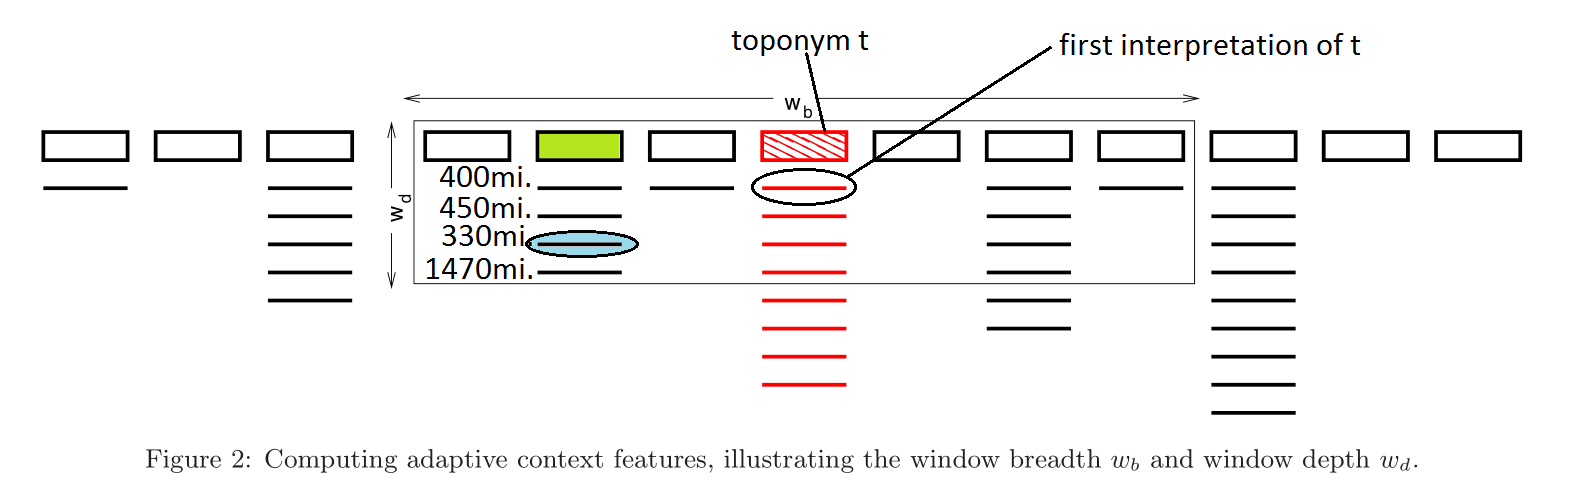
\includegraphics[width=\textwidth]{adaptive-proximity-i.png} 
			\caption{from Lieberman and Samet, \textit{Source: URL}}
		\end{figure}
		
		\onslide<11>
		\begin{figure}
			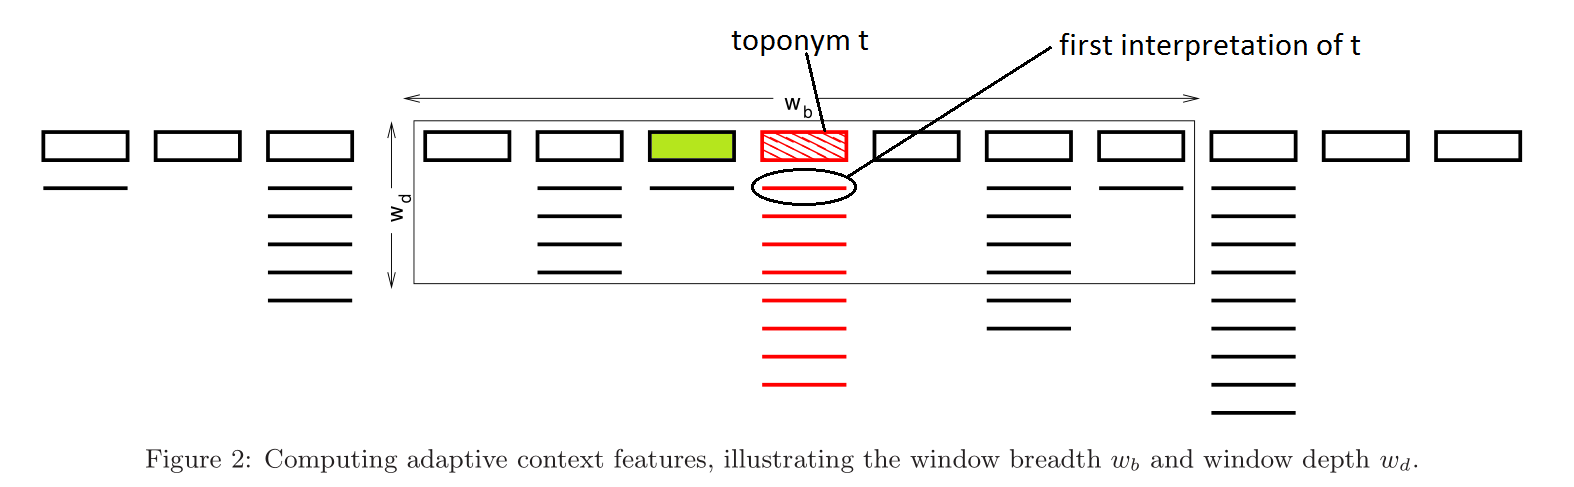
\includegraphics[width=\textwidth]{adaptive-proximity-j.png} 
			\caption{from Lieberman and Samet, \textit{Source: URL}}
		\end{figure}
		
		\onslide<12>
		\begin{figure}
			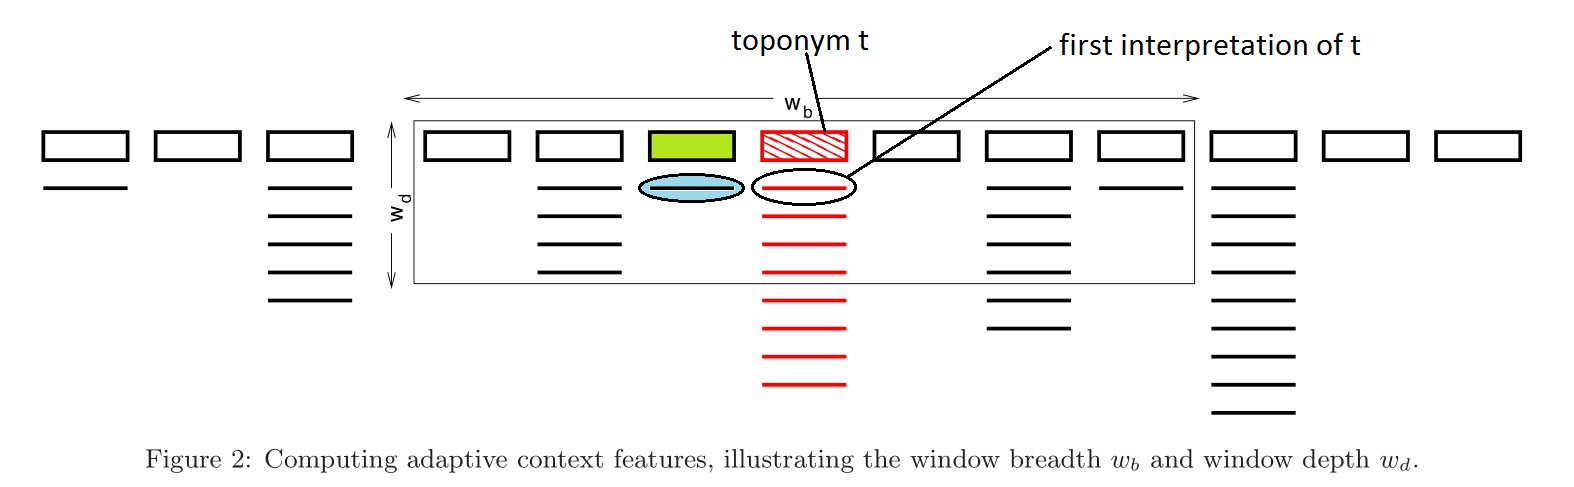
\includegraphics[width=\textwidth]{adaptive-proximity-j1.png} 
			\caption{from Lieberman and Samet, \textit{Source: URL}}
		\end{figure}
		
		\onslide<13>
		\begin{figure}
			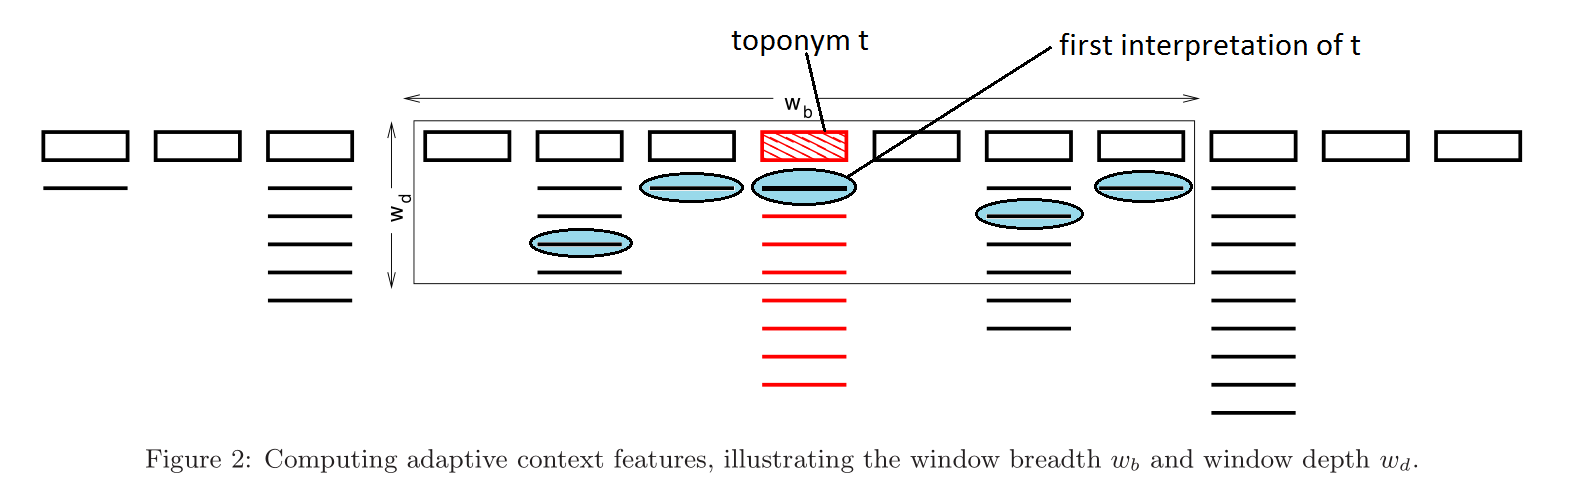
\includegraphics[width=\textwidth]{adaptive-proximity-k.png} 
			\caption{from Lieberman and Samet, \textit{Source: URL}}
		\end{figure}
		
		\onslide<14>
		\begin{figure}
			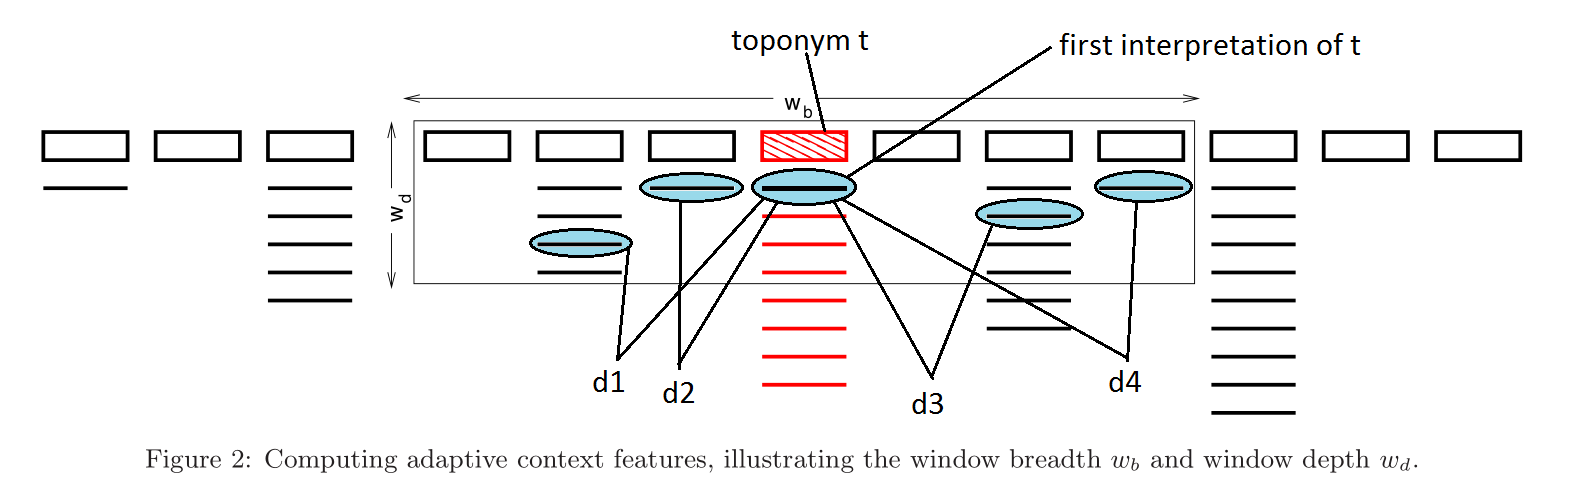
\includegraphics[width=\textwidth]{adaptive-proximity-k1.png} 
			\caption{from Lieberman and Samet, \textit{Source: URL}}
		\end{figure}
		
		\onslide<15>
		\begin{figure}
			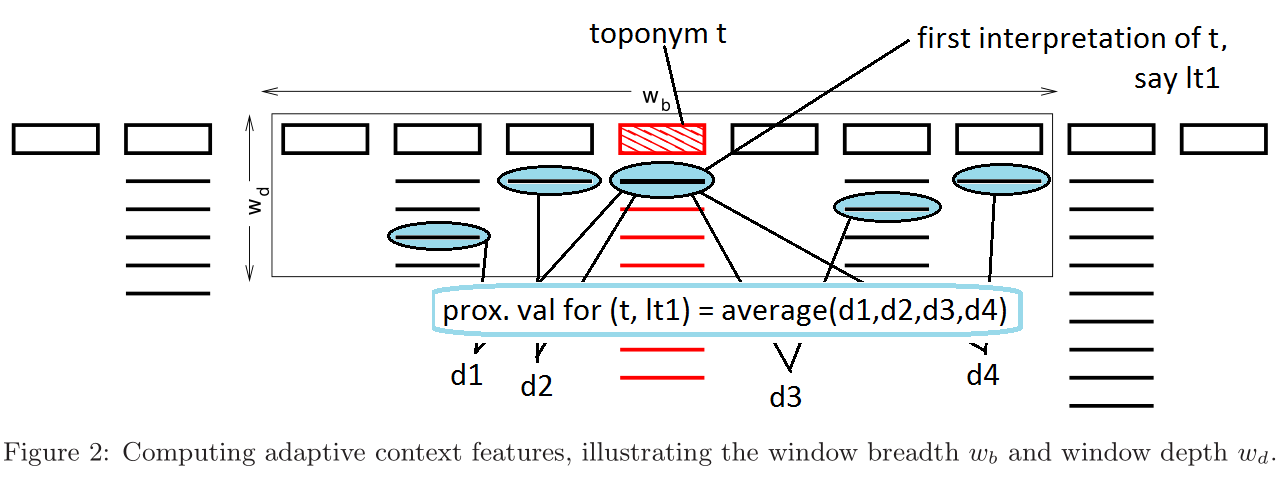
\includegraphics[width=\textwidth]{adaptive-proximity-k2.png} 
			\caption{from Lieberman and Samet, \textit{Source: URL}}
		\end{figure}
		
		\onslide<16>
		\begin{figure}
			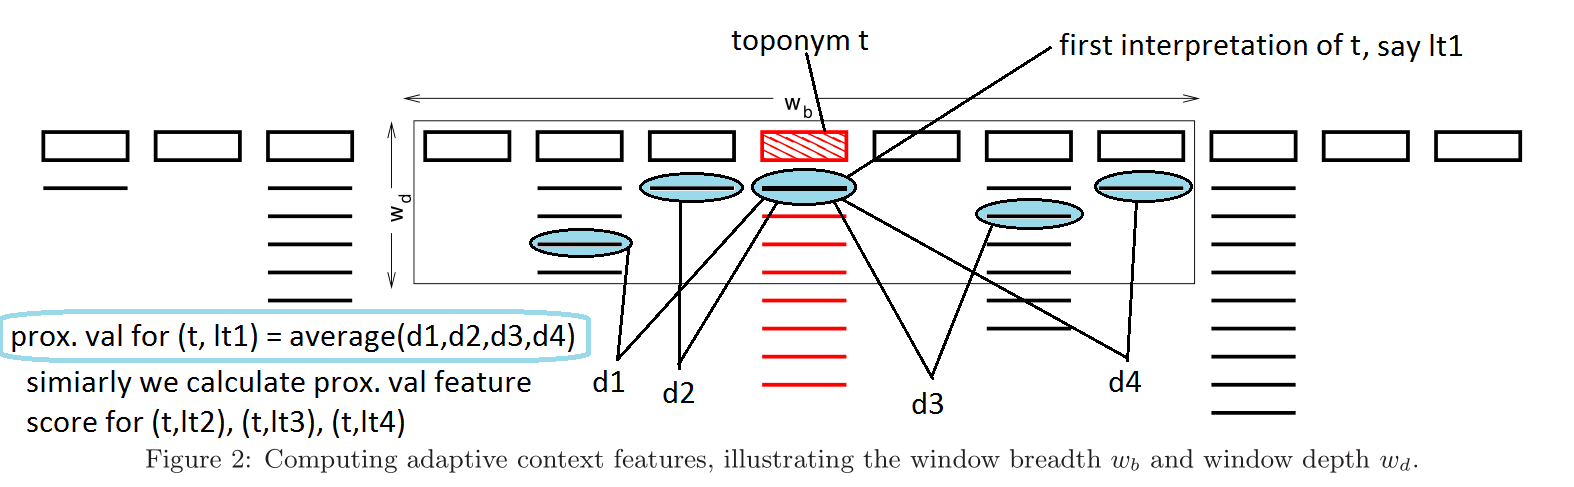
\includegraphics[width=\textwidth]{adaptive-proximity-k3.png} 
			\caption{from Lieberman and Samet, \textit{Source: URL}}
		\end{figure}
		
		\onslide<17>
		\begin{figure}
			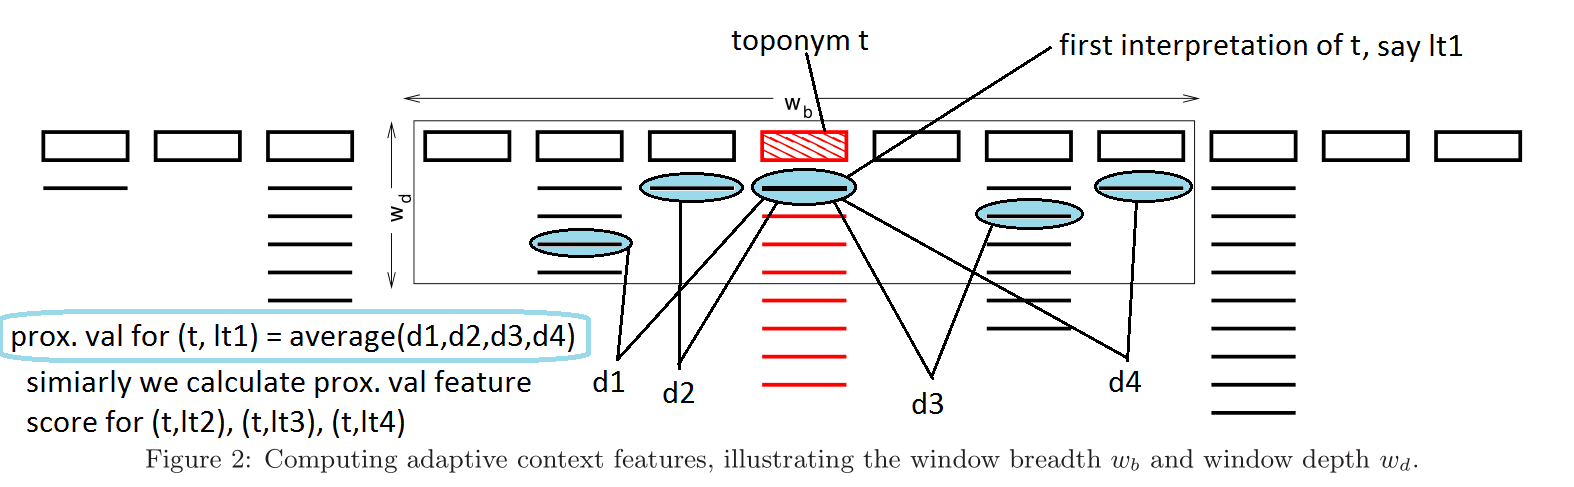
\includegraphics[width=\textwidth]{adaptive-proximity-k3.png} 
			\caption{from Lieberman and Samet, \textit{Source: URL}}
		\end{figure}
		
		\vspace*{-5cm}
		\begin{block}{\centering Proximity features}
			\centering  \textbf{the interpretation $l_t$, for which proximity score is lowest, is the chosen as the correct interpretation of $t$}
		\end{block}
		
	\end{overprint}
} % END OF FRAME
%----------------------------------------

\subsection{Proximity Features idea}
\frame{
	\frametitle{Proximity Features idea}
	
\begin{block}{\centering Proximity features}
	\centering  \textbf{all toponyms $o$ in the window around $t$ play a role in determining correct interpretation $l_t$ of $t$}
\end{block}

\pause

\begin{block}{\centering News articles}
	\centering  \textbf{generally talk about a specific region, so a news article will have many proximate toponyms}
\end{block}

	
} % END OF FRAME

%----------------------------------------

\frame{
	\frametitle{Proximity Features - example}
	
	``...,	Birmingham and Perth. It was relatively warm in London ...''
	
	\pause
	
	Assuming $w_d$=2, 
	
		\begin{tabular}{ c| c | c | c}
		{} & Birmingham & \textbf{Perth} & London \\
		\hline
		1 & UK & Scotland & UK \\
		2 & Michigan, USA & Australia & Ontario, Canada \\
		\end{tabular}
	
	\pause
	
		\begin{tabular}{c l l}
		$\checkmark$ & (Perth, Scotland) $\xrightarrow{distance}$ (Birmingham, UK) & 338.8 miles\\
		{} & (Perth, Scotland) $\xrightarrow{distance}$ (Birmingham, Michigan) & 3496.2 miles \\
		$\checkmark$ & (Perth, Scotland) $\xrightarrow{distance}$ (London, UK) & 450.6 miles \\
		{} & (Perth, Scotland) $\xrightarrow{distance}$ (London, Ontario) & 3403.7 miles \\
		\end{tabular} \\
		
		prox score(Perth, Scotland) = average(338.8, 450.6) = 394.7\footnotemark miles \\
				
	\only<2->{\footnotetext[1]{The authors used geometric median for average}}
		
	\vfill
} % END OF FRAME

%----------------------------------------
\subsection{Proximity Features - example}
\frame{
	\frametitle{Proximity Features - example}
	
	``...,	Birmingham and Perth. It was relatively warm in London ...''
	
	\pause
	
	Assuming $w_d$=2, 
	
	\begin{tabular}{ c| c | c | c}
	{} & Birmingham & \textbf{Perth} & London \\
	\hline
	1 & UK & Scotland & UK \\
	2 & Michigan, USA & Australia & Ontario, Canada \\
	\end{tabular}
	
	\pause
	
	prox score(Perth, Scotland) = average(338.8, 450.6) = 394.7\footnotemark[1] miles  \\
	
	\pause
	
	similarly we calculate prox score for second $(t, l_t)$ pair  \\
	
	
	\begin{tabular}{c l l}
	$\checkmark$ & (Perth, Australia) $\xrightarrow{distance}$ (Birmingham, UK) & 9085 miles\\
	{} & (Perth, Australia) $\xrightarrow{distance}$ (Birmingham, Michigan) & 11,175 miles \\
	$\checkmark$ & (Perth, Australia) $\xrightarrow{distance}$ (London, UK) & 9007 miles \\
	{} & (Perth, Australia) $\xrightarrow{distance}$ (London, Ontario) & 11,245 miles \\
	\end{tabular} \\
	
	
	
	\pause
	
	prox score(Perth, Australia) = average(9085, 9007) = 9046\footnotemark[1] miles  \\
	
	\pause
	
	\begin{overprint}
		\vspace*{-3cm}
		\begin{block}{\centering Proximity features}
			\centering \textbf{So the correct interp. for Perth, in this context, using Prox feature only would be (Perth, Scotland)!} \\
			\centering \textbf{as prox score(Perth, Scotland) \textless prox score(Perth, Australia)}
		\end{block}
	\end{overprint}
	
	

	
	
	\only<2->{\footnotetext[1]{The authors used geometric median for average}}
	

	\vfill
} % END OF FRAME
%----------------------------------------


\subsection{2. Sibling Features}
\frame{
	\frametitle{2. Sibling Features}
	
	\begin{block}{2. Sibling Features}
		capture the toponyms that belong to same country, state	or any other administrative division
	\end{block}
	
	\pause
	
	\begin{itemize}
		\item capture sibling relations
		\item capture containment relationships 
	\end{itemize}
	
	\pause
	
	e.g. ``Saarbruecken and Voelklingen" are siblings at city level \\
	
	\pause
	
	e.g. "Paris, Texas" refers to Paris in Texas, USA \\
	
	\pause
	
	\textbf{computed in a similar way as the proximity features!}
	
} % END OF FRAME
%----------------------------------------

\subsection{Sibling Features idea}
\frame{
	\frametitle{Sibling Features idea}
	
	\begin{block}{\centering Sibling features}
		\centering  \textbf{play a role in determining correct interpretation for cities that are geographically far away but have common parent such as state or country}
	\end{block}
	
	\pause
	
	\begin{block}{\centering Sibling features}
		\centering  \textbf{can correctly capture relationships which may be considered geographically distant}
	\end{block}
	
	\vfill
} % END OF FRAME
%----------------------------------------

\subsection{Sibling Features - example}
\frame{
	\frametitle{Sibling Features - example}
	
	``... Bloomington, Rochester and Duluth. ..."
	
	\pause
	
	Assuming $w_d$=3, 
	
	\begin{tabular}{ c| c | c | c}
		
		{} & Bloomington & \textbf{Rochester} & Duluth \\
		\hline
		1 & Minnesota, USA & Victoria, Australia & Georgia, USA\\
		2 & Michigan, USA & New York, USA & Minnesota, USA\\
		2 & {} & Minnesota, USA & {}\\
	\end{tabular} \\
	
	... \\
	\pause
	
	
	\textbf{The sibling feature scores for toponym/interp pairs will be}
	\begin{tabular}{ c| c | c | c}
		
		{} & $(t, l_t)$ & Score & common sibling levels. \\
		\hline
		1 & (Rochester, Victoria Australia) & 0 & -\\
		2 & (Rochester, New York USA) & 4 & 4 x USA\\
		2 & (Rochester, Minnesota USA) & 6 & 4 x USA, 2 x Minnesota\\
	\end{tabular}
	
	\vfill
} % END OF FRAME
%----------------------------------------

\subsection{Evaluation measures}
\frame{
	\frametitle{Evaluation measures}
	
	\begin{itemize}
		\item Precision
		\item Recall
		\item F1 score
	\end{itemize}
	
	\pause

	Precision = $\frac{\text{no. of correctly resolved toponyms}}{\text{no. of total resolved toponyms}}$ \\
	...\\
	Recall = $\frac{\text{no. of correctly resolved toponyms}}{\text{no. of true toponyms}}$
} % END OF FRAME
%----------------------------------------


\subsection{Evaluation results}
\frame{
	\frametitle{Evaluation results}
	
	\begin{itemize}
		\item  news data from ACE, LGL and CLUST datasets
		\item  compared with two commercial geotagging frameworks i.e. (Thomson Reuter's OpenCalais and Yahoo!'s Placemaker)
	\end{itemize}
	
	\pause
	
	\textbf{performed better in majority of test scenarios and datasets} \\
	
	(details in the original paper)
	
} % END OF FRAME
%----------------------------------------


%========================================
%========================================

\section[Applications]{Applications}

%\subsection{Highlighting}

%----------------------------------------

\def\hilite<#1>{%
	\temporal<#1>{\color{black}}{\color{MPIIred}}%
	{\color{gray}}}

%----------------------------------------

\subsection{Geographic visualization and browsing}
\frame{
	\frametitle{Geographic visualization and browsing}
	
	\begin{itemize}
		\item thematic maps
		\item geographic anchoring of encyclopedia articles
	\end{itemize}
		
} % END OF FRAME

%----------------------------------------

\subsection{Question answering}
\frame{
	\frametitle{Question answering}
	
	\textbf{trend in search engines to answer some questions directly, instead of returning search results} \\
	
	\pause
	
	e.g. consider the query ``What is the distance between between Lahore and Multan?" \\
	...\\
	
	\pause
	
	can be solved by
	\begin{itemize}
		\item (1) resolve both toponyms in the query, 
		\item (2) compute the geographic distance using a geometric formula
	\end{itemize}
	
} % END OF FRAME

%----------------------------------------

\subsection{Improving search results}
\frame{
	\frametitle{Improving search results - for geographic queries}
	
	\textbf{return relevant documents which would not be returned using keyword based search} \\
	...\\
	
	\pause
	
	e.g. query is "Saarland" \\
	
	should also return documents which mention cities of Saarland, but not the keyword \textbf{Saarland} in them! \\
	...\\
	\pause
	
	\textbf{can be done by assigning geographic focus to documents}
	
} % END OF FRAME


%----------------------------------------

\subsection{Browsing news geographically}
\frame{
	\frametitle{Browsing news geographically}
	
	
	e.g. system \textbf{NewsStand System: }	
	users can choose a region of interest and read news and articles relevant to it\\
	or browse news geographically on world map in  an interactive manner
	\pause
	\bigskip
	\begin{itemize}
		\item crawls around 50,000 news article every day
		\item cluster them on content and location
		\item associate each cluster to its geographic focus
		\item stories appear as the map as the map is zoomed in/out
	\end{itemize}
	
} % END OF FRAME

%----------------------------------------

\subsection{Browsing news geographically - NewsStand}
\frame{
	\frametitle{Browsing news geographically - NewsStand}
	
	
	\begin{overprint}
		\onslide<1>
		\begin{figure}
			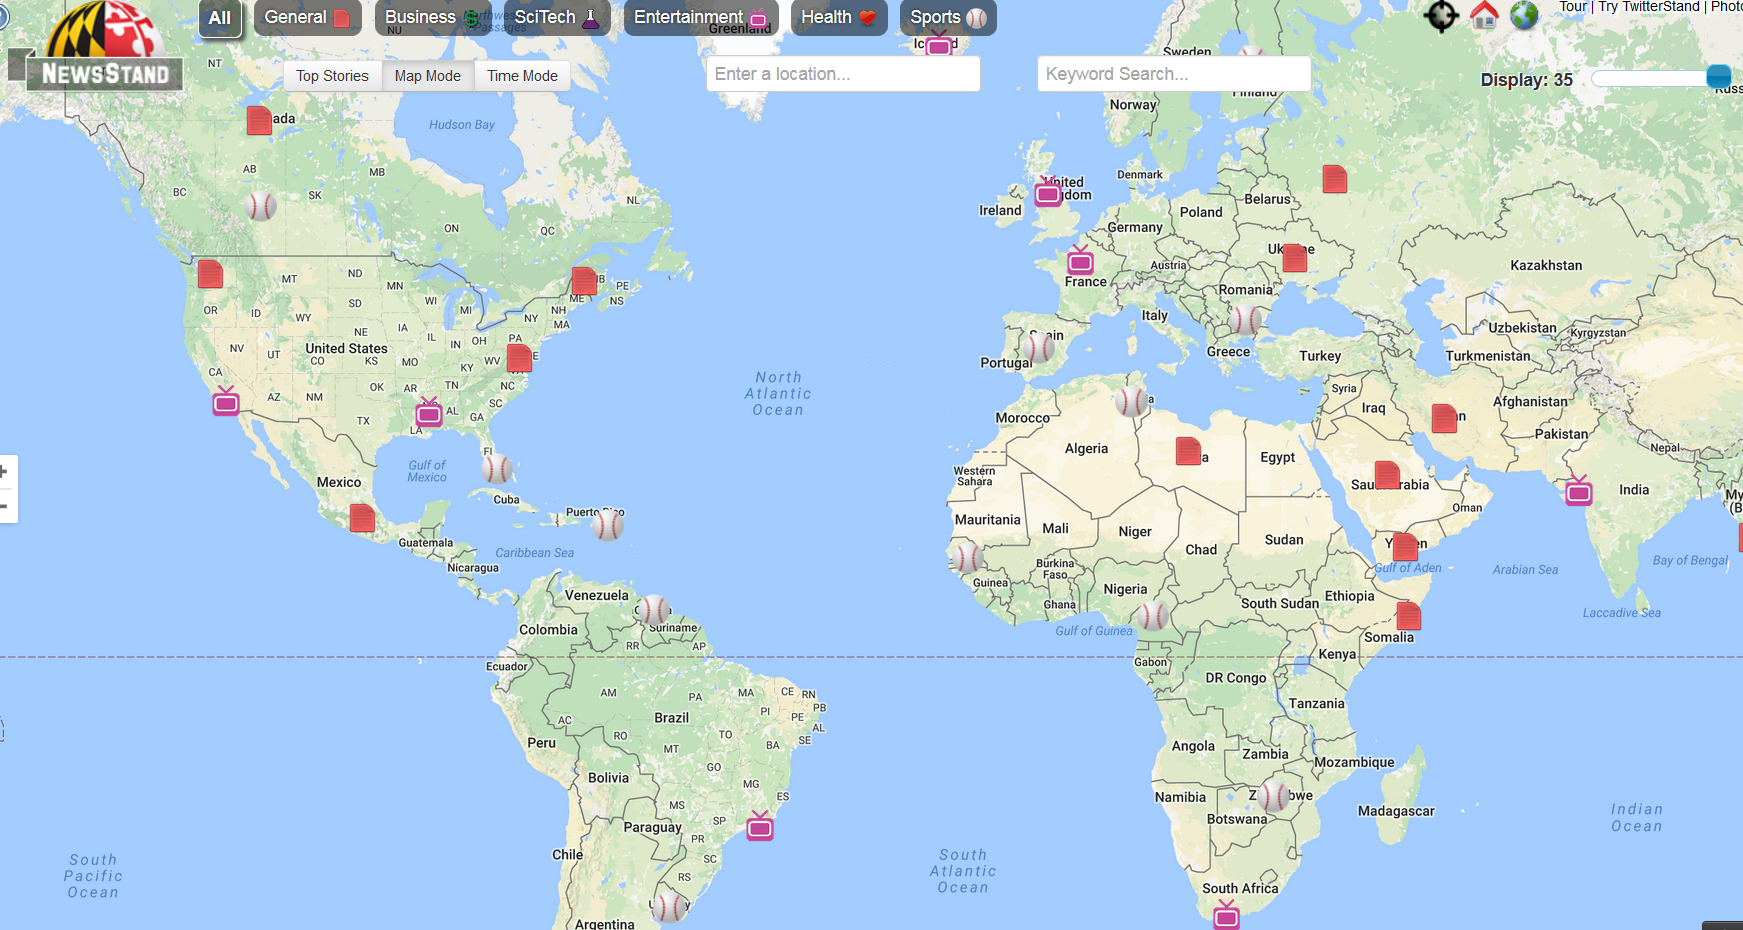
\includegraphics[width=\textwidth]{aus0.png} 
			\caption{NewsStand System, \textit{Source: URL}}
		\end{figure}
		
		\onslide<2>
		\begin{figure}
			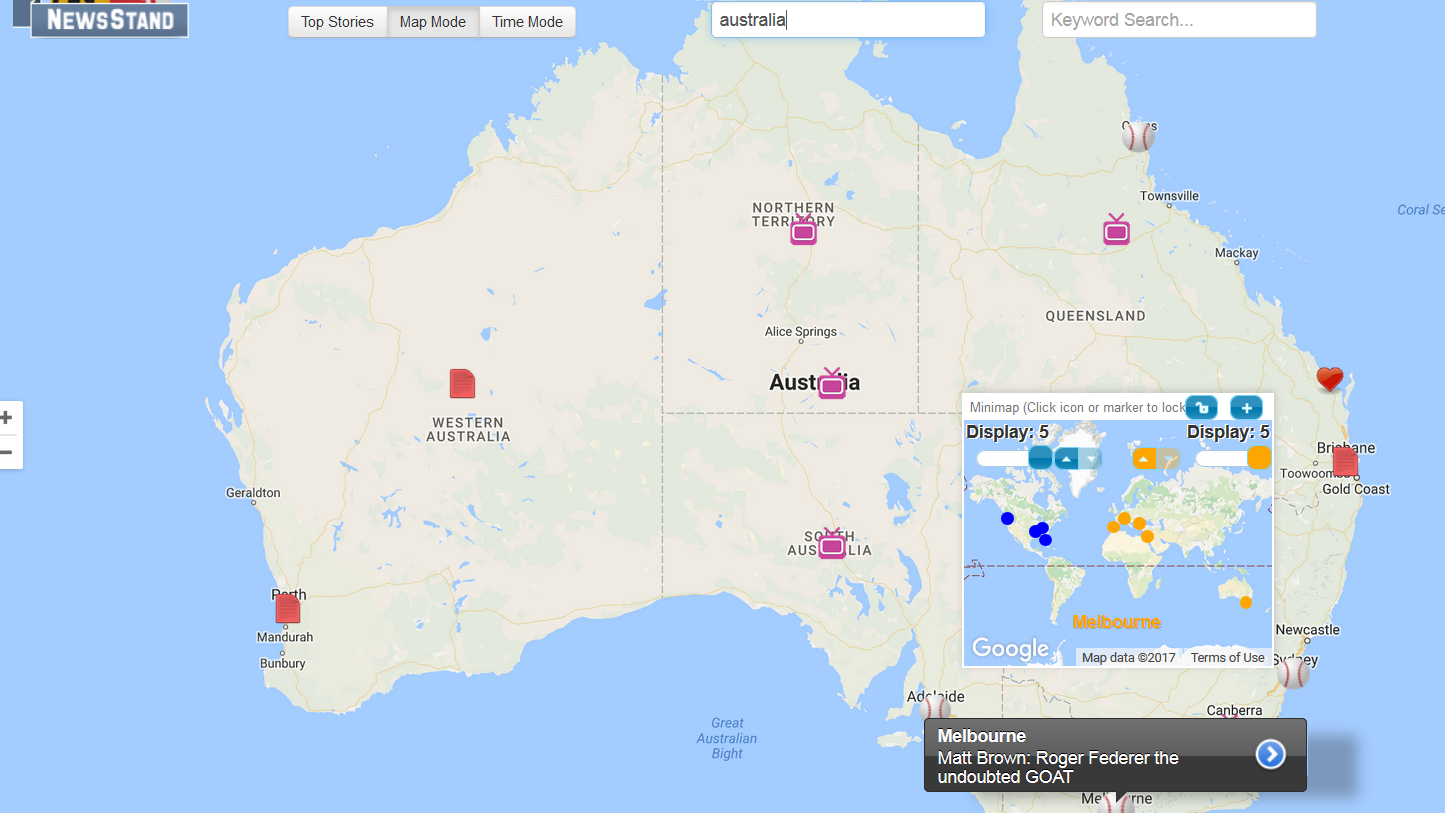
\includegraphics[width=\textwidth]{aus1.png} 
			\caption{NewsStand System, \textit{Source: URL}}
		\end{figure}
		
		\onslide<3>
		\begin{figure}
			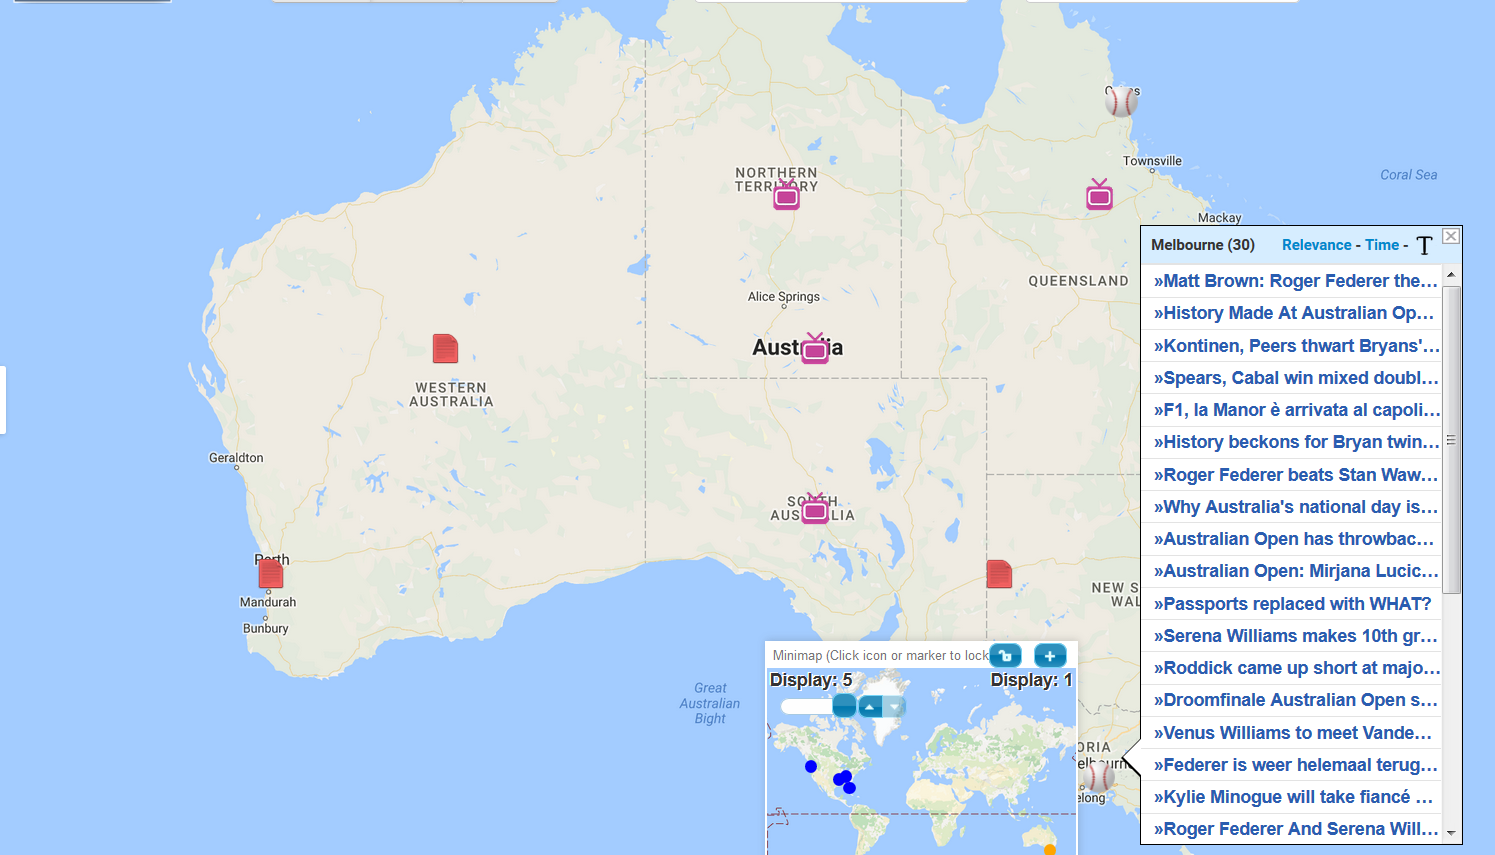
\includegraphics[width=\textwidth]{aus2.png} 
			\caption{NewsStand System, \textit{Source: URL}}
		\end{figure}
	\end{overprint}
	
	\vfill
} % END OF FRAME
%========================================
%========================================



\section[Conclusion]{Conclusion}
\subsection{Conclusion}
\frame{
	\frametitle{Conclusion}
	
	\begin{itemize}
		\item Geotagging an important process which allows to
		\begin{itemize}
			\item find toponyms (Recognition)
			\item resolve/ground them (Resolution)
		\end{itemize}
		\item existing NER techniques can help in recognition
		\item many features can be used to help in resolution
		\item geotagging has many applications/usecases
	\end{itemize}
		
} % END OF FRAME


%----------------------------------------

\frame{\frametitle{Questions}

\begin{center}\begin{LARGE}\textbf{Questions?}\end{LARGE}\end{center}


}

\newcommand{\backupbegin}{
   \newcounter{framenumberappendix}
   \setcounter{framenumberappendix}{\value{framenumber}}
}
\newcommand{\backupend}{
   \addtocounter{framenumberappendix}{-\value{framenumber}}
   \addtocounter{framenumber}{\value{framenumberappendix}} 
}

\appendix
\backupbegin


\backupend

\end{document}
